\documentclass{standalone}
\usepackage{tikz}
\usetikzlibrary{patterns, positioning}


\begin{document}
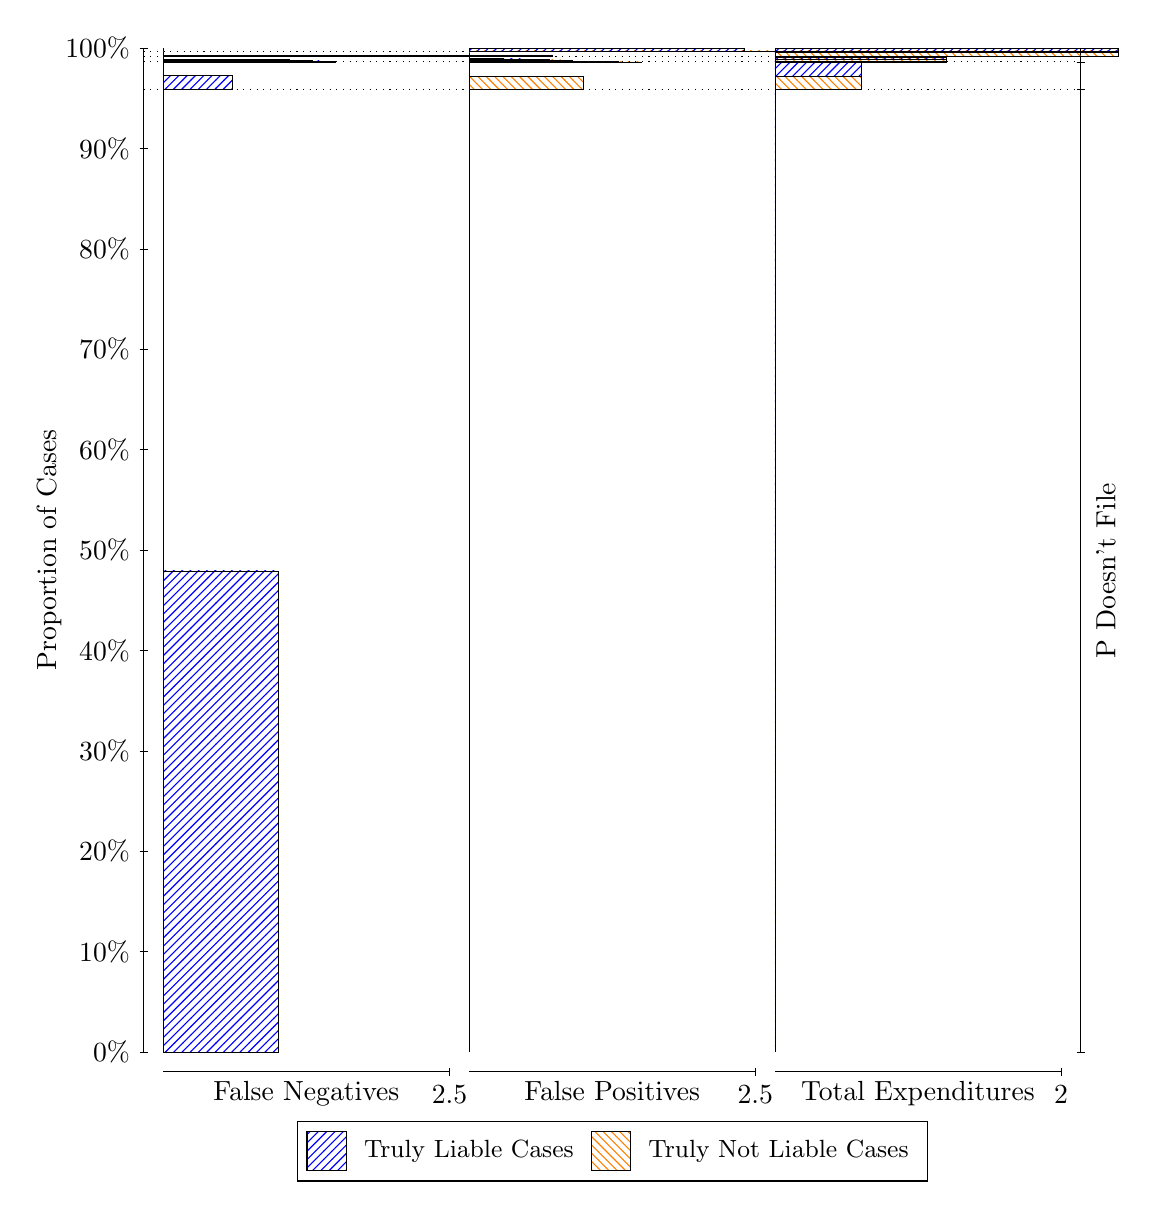
\begin{tikzpicture}
\draw[black, very thin] (1.5,1.75) -- (1.5,14.5);
\node[rotate=90, text=black, anchor=center] at (0.3, 8.125) {Proportion of Cases};
\draw[black, very thin] (1.45,1.75) -- (1.55,1.75);
\node[text=black, anchor=east] at (1.45, 1.75) {0\%};
\draw[black, very thin] (1.45,3.025) -- (1.55,3.025);
\node[text=black, anchor=east] at (1.45, 3.025) {10\%};
\draw[black, very thin] (1.45,4.3) -- (1.55,4.3);
\node[text=black, anchor=east] at (1.45, 4.3) {20\%};
\draw[black, very thin] (1.45,5.575) -- (1.55,5.575);
\node[text=black, anchor=east] at (1.45, 5.575) {30\%};
\draw[black, very thin] (1.45,6.85) -- (1.55,6.85);
\node[text=black, anchor=east] at (1.45, 6.85) {40\%};
\draw[black, very thin] (1.45,8.125) -- (1.55,8.125);
\node[text=black, anchor=east] at (1.45, 8.125) {50\%};
\draw[black, very thin] (1.45,9.4) -- (1.55,9.4);
\node[text=black, anchor=east] at (1.45, 9.4) {60\%};
\draw[black, very thin] (1.45,10.675) -- (1.55,10.675);
\node[text=black, anchor=east] at (1.45, 10.675) {70\%};
\draw[black, very thin] (1.45,11.95) -- (1.55,11.95);
\node[text=black, anchor=east] at (1.45, 11.95) {80\%};
\draw[black, very thin] (1.45,13.225) -- (1.55,13.225);
\node[text=black, anchor=east] at (1.45, 13.225) {90\%};
\draw[black, very thin] (1.45,14.5) -- (1.55,14.5);
\node[text=black, anchor=east] at (1.45, 14.5) {100\%};

\draw[black, very thin] (13.4,1.75) -- (13.4,14.5);
\draw[black, very thin] (13.35,1.75) -- (13.45,1.75);
\node[anchor=west] at (13.35, 1.75) {};
\draw[black, very thin] (13.35,13.97) -- (13.45,13.97);
\node[anchor=west] at (13.35, 13.97) {};
\draw[black, very thin] (13.35,14.324) -- (13.45,14.324);
\node[anchor=west] at (13.35, 14.324) {};
\draw[black, very thin] (13.35,14.393) -- (13.45,14.393);
\node[anchor=west] at (13.35, 14.393) {};
\draw[black, very thin] (13.35,14.454) -- (13.45,14.454);
\node[anchor=west] at (13.35, 14.454) {};
\draw[black, very thin] (13.35,14.5) -- (13.45,14.5);
\node[anchor=west] at (13.35, 14.5) {};

\draw[black, very thin, pattern color=blue, pattern=north east lines] (1.75,1.75) rectangle (3.2033,7.8599);
\draw[black, very thin, pattern color=orange, pattern=north west lines] (1.75,7.8599) rectangle (1.75,13.97);
\draw[black, very thin, pattern color=blue, pattern=north east lines] (1.75,13.97) rectangle (2.622,14.157);
\draw[black, very thin, pattern color=orange, pattern=north west lines] (1.75,14.157) rectangle (1.75,14.324);
\draw[black, very thin, pattern color=blue, pattern=north east lines] (1.75,14.324) rectangle (3.93,14.331);
\draw[black, very thin, pattern color=blue, pattern=north east lines] (1.75,14.331) rectangle (3.7847,14.336);
\draw[black, very thin, pattern color=blue, pattern=north east lines] (1.75,14.336) rectangle (3.6393,14.343);
\draw[black, very thin, pattern color=blue, pattern=north east lines] (1.75,14.343) rectangle (3.494,14.346);
\draw[black, very thin, pattern color=blue, pattern=north east lines] (1.75,14.346) rectangle (3.3487,14.351);
\draw[black, very thin, pattern color=blue, pattern=north east lines] (1.75,14.351) rectangle (3.2033,14.352);
\draw[black, very thin, pattern color=blue, pattern=north east lines] (1.75,14.352) rectangle (3.058,14.354);
\draw[black, very thin, pattern color=blue, pattern=north east lines] (1.75,14.354) rectangle (2.9127,14.355);
\draw[black, very thin, pattern color=blue, pattern=north east lines] (1.75,14.355) rectangle (2.7673,14.356);
\draw[black, very thin, pattern color=orange, pattern=north west lines] (1.75,14.356) rectangle (1.75,14.393);
\draw[black, very thin, pattern color=blue, pattern=north east lines] (1.75,14.393) rectangle (6.6913,14.403);
\draw[black, very thin, pattern color=orange, pattern=north west lines] (1.75,14.403) rectangle (1.75,14.454);
\draw[black, very thin, pattern color=orange, pattern=north west lines] (1.75,14.454) rectangle (1.75,14.464);
\draw[black, very thin, pattern color=blue, pattern=north east lines] (1.75,14.464) rectangle (1.75,14.5);
\draw[black, very thin, pattern color=orange, pattern=north west lines] (5.6333,1.75) rectangle (5.6333,7.86);
\draw[black, very thin, pattern color=blue, pattern=north east lines] (5.6333,7.86) rectangle (5.6333,13.97);
\draw[black, very thin, pattern color=orange, pattern=north west lines] (5.6333,13.97) rectangle (7.0867,14.137);
\draw[black, very thin, pattern color=blue, pattern=north east lines] (5.6333,14.137) rectangle (5.6333,14.324);
\draw[black, very thin, pattern color=orange, pattern=north west lines] (5.6333,14.324) rectangle (7.8133,14.325);
\draw[black, very thin, pattern color=orange, pattern=north west lines] (5.6333,14.325) rectangle (7.668,14.325);
\draw[black, very thin, pattern color=orange, pattern=north west lines] (5.6333,14.325) rectangle (7.5227,14.327);
\draw[black, very thin, pattern color=orange, pattern=north west lines] (5.6333,14.327) rectangle (7.3773,14.329);
\draw[black, very thin, pattern color=orange, pattern=north west lines] (5.6333,14.329) rectangle (7.232,14.332);
\draw[black, very thin, pattern color=orange, pattern=north west lines] (5.6333,14.332) rectangle (7.0867,14.334);
\draw[black, very thin, pattern color=orange, pattern=north west lines] (5.6333,14.334) rectangle (6.9413,14.342);
\draw[black, very thin, pattern color=orange, pattern=north west lines] (5.6333,14.342) rectangle (6.796,14.35);
\draw[black, very thin, pattern color=orange, pattern=north west lines] (5.6333,14.35) rectangle (6.6507,14.36);
\draw[black, very thin, pattern color=blue, pattern=north east lines] (5.6333,14.36) rectangle (6.36,14.361);
\draw[black, very thin, pattern color=blue, pattern=north east lines] (5.6333,14.361) rectangle (6.2147,14.362);
\draw[black, very thin, pattern color=blue, pattern=north east lines] (5.6333,14.362) rectangle (6.0693,14.364);
\draw[black, very thin, pattern color=blue, pattern=north east lines] (5.6333,14.364) rectangle (5.924,14.366);
\draw[black, very thin, pattern color=blue, pattern=north east lines] (5.6333,14.366) rectangle (5.7787,14.37);
\draw[black, very thin, pattern color=blue, pattern=north east lines] (5.6333,14.37) rectangle (5.6333,14.393);
\draw[black, very thin, pattern color=orange, pattern=north west lines] (5.6333,14.393) rectangle (5.6333,14.444);
\draw[black, very thin, pattern color=blue, pattern=north east lines] (5.6333,14.444) rectangle (5.6333,14.454);
\draw[black, very thin, pattern color=orange, pattern=north west lines] (5.6333,14.454) rectangle (10.575,14.464);
\draw[black, very thin, pattern color=blue, pattern=north east lines] (5.6333,14.464) rectangle (9.1213,14.5);
\draw[black, very thin, pattern color=orange, pattern=north west lines] (9.5167,1.75) rectangle (9.5167,7.86);
\draw[black, very thin, pattern color=blue, pattern=north east lines] (9.5167,7.86) rectangle (9.5167,13.97);
\draw[black, very thin, pattern color=orange, pattern=north west lines] (9.5167,13.97) rectangle (10.607,14.137);
\draw[black, very thin, pattern color=blue, pattern=north east lines] (9.5167,14.137) rectangle (10.607,14.324);
\draw[black, very thin, pattern color=orange, pattern=north west lines] (9.5167,14.324) rectangle (11.697,14.327);
\draw[black, very thin, pattern color=blue, pattern=north east lines] (9.5167,14.327) rectangle (11.697,14.331);
\draw[black, very thin, pattern color=orange, pattern=north west lines] (9.5167,14.331) rectangle (11.697,14.362);
\draw[black, very thin, pattern color=blue, pattern=north east lines] (9.5167,14.362) rectangle (11.697,14.387);
\draw[black, very thin, pattern color=orange, pattern=north west lines] (9.5167,14.387) rectangle (11.697,14.39);
\draw[black, very thin, pattern color=blue, pattern=north east lines] (9.5167,14.39) rectangle (11.697,14.393);
\draw[black, very thin, pattern color=orange, pattern=north west lines] (9.5167,14.393) rectangle (13.877,14.444);
\draw[black, very thin, pattern color=blue, pattern=north east lines] (9.5167,14.444) rectangle (13.877,14.454);
\draw[black, very thin, pattern color=orange, pattern=north west lines] (9.5167,14.454) rectangle (13.877,14.464);
\draw[black, very thin, pattern color=blue, pattern=north east lines] (9.5167,14.464) rectangle (13.877,14.5);
\draw[black, dotted] (1.5,13.97) -- (13.4,13.97);
\draw[black, dotted] (1.5,14.324) -- (13.4,14.324);
\draw[black, dotted] (1.5,14.393) -- (13.4,14.393);
\draw[black, dotted] (1.5,14.454) -- (13.4,14.454);
\draw[black, very thin] (1.75,1.5) -- (5.3833,1.5);
\node[text=black, anchor=north] at (3.5667, 1.5) {False Negatives};
\draw[black, very thin] (5.3833,1.45) -- (5.3833,1.55);
\node[text=black, anchor=north] at (5.3833, 1.45) {2.5};

\draw[black, very thin] (5.6333,1.5) -- (9.2667,1.5);
\node[text=black, anchor=north] at (7.45, 1.5) {False Positives};
\draw[black, very thin] (9.2667,1.45) -- (9.2667,1.55);
\node[text=black, anchor=north] at (9.2667, 1.45) {2.5};

\draw[black, very thin] (9.5167,1.5) -- (13.15,1.5);
\node[text=black, anchor=north] at (11.333, 1.5) {Total Expenditures};
\draw[black, very thin] (13.15,1.45) -- (13.15,1.55);
\node[text=black, anchor=north] at (13.15, 1.45) {2};

\node[text=black, centered, rotate=90] at (13.72, 7.8599) {P Doesn't File};





\draw (7.449999999999999,1.5) node[draw=none] (baseCoordinate) {};
\begin{scope}[align=center]
        \matrix[scale=0.5, draw=black, below=0.5cm of baseCoordinate, nodes={draw}, column sep=0.1cm]{
            \node[rectangle, draw, minimum width=0.5cm, minimum height=0.5cm, pattern color=blue, pattern=north east lines] {}; &
            \node[draw=none, font=\small, text=black] (B) {Truly Liable Cases}; &
            \node[rectangle, draw, minimum width=0.5cm, minimum height=0.5cm, pattern color=orange, pattern=north west lines] {}; &
            \node[draw=none, font=\small, text=black] (B) {Truly Not Liable Cases}; \\
            };
\end{scope}

\end{tikzpicture}
\end{document}